\subsection{RR}
\label{subsection:RR}
%% pourquoi (tester firefox), comment (ordre des threads -> perf API dans le CPU)

La plus grande partie de l'exécution d'une application est
déterministe. Néanmoins, il reste des instructions non déterministes entraînant
un exécution toujours différente de l'application (signaux, adresses de
buffers...). Elles peuvent conduire à des fautes qui sont persistantes ou qui
apparaissent après un certain nombre d'exécutions ou qui sont totalement
aléatoires et peuvent ne pas réapparaître lors de la réexécution de
l'application. Essayer de résoudre ces bugs de façon conventionnelle étant très
difficile, il faut trouver de nouvelles méthodes. C'est pour cela que RR a été
créé. RR \citep{RR} est outil de débogage utilisant l'émulation par interception
et qui vise à surpasser gdb. Il a été créé pour déboguer Firefox, mais il
peut-être utilisé sur n'importe quel type d'application. Il résout le problème
des exécutions non déterministes en deux phases. La première consiste à
enregistrer l'exécution de tous les événements non déterministes qui pourraient
échouer. La seconde débogue l'exécution de façon déterministe en rejouant
l'enregistrement aussi souvent qu'on le souhaite. On relance toujours la même
exécution et les ressources restent les mêmes (espace d'adressage, contenu
des registres, appels système), d'où l'idée de déterminisme. Avec cette
méthode, on peut même déboguer les fautes qui sont produites par des outils de
fuzzing\footnote{ Technique pour tester des logiciels basée sur l'injection des
  données aléatoires dans les entrées d'un programme. Si le programme échoue:
  plantage ou génération d'erreur, alors il y a des défauts à
  corriger. \\ \url{http://fr.wikipedia.org/wiki/Fuzzing}} ou d'injection de
fautes. Néanmoins, pour des raisons d'efficacité RR ne sauvegarde pas la mémoire
partagée lors d'exécutions multi-thread. Ce choix permet de n'émuler qu'une
machine mono-c\oe ur qui est plus simple à gérer même si cela empêche le
parallélisme.

RR utilise différents outils selon la phase de son
exécution\citep{RRimplem}. Dans la phase d'enregistrement, pour gérer
l'ordonnancement lors du rejeu, il sauvegarde les actions qu'il considère comme
mécanisme d'interruption d'une application: \textit{i)} les appels système
exécutés \textit{ii)} la préemption via HPC\footnote{Hardware Performance
  Counters \\ On compte les instructions qui s'exécutent et on arrête
  l'application quand le nombre d'instrucions exécuté atteint la valeur du HPC
  fournie par l'utilisateur.} en sauvegardant le nombre d'instructions à exécuter
avant une interruption \textit{iii)} les signaux UNIX exécutés ainsi que leur
handler s'il est réimplémenté. Dans la phase de rejeu, RR utilise les données
non déterministes sauvegardées lors de la première phase pour mettre en place
son émulation (appels système, compteur d'instructions, handler de signal,
valeur des registres lors de ces actions). Quand RR va rejouer un appel système,
les valeurs de retour des registres seront celles sauvegardées lors de
l'exécution réelle et non celles du rejeu. Pour intercepter les appels système,
RR utilise \texttt{LD\_PRELOAD} (section \ref{paragraphe:LDPreload}) qui va les
placer dans un buffer. Ensuite Seccomp/BPF(section\ref{paragraph:seccomp/bpf})
parcourra le buffer pour filtrer les appels système et les laisser
exécuter. Pour cette partie de la gestion de l'appel on n'utilise pas ptrace car
il est trop couteux en terme de changement de contexte, Figure \ref{AS_RR}.
\begin{figure}
\centering 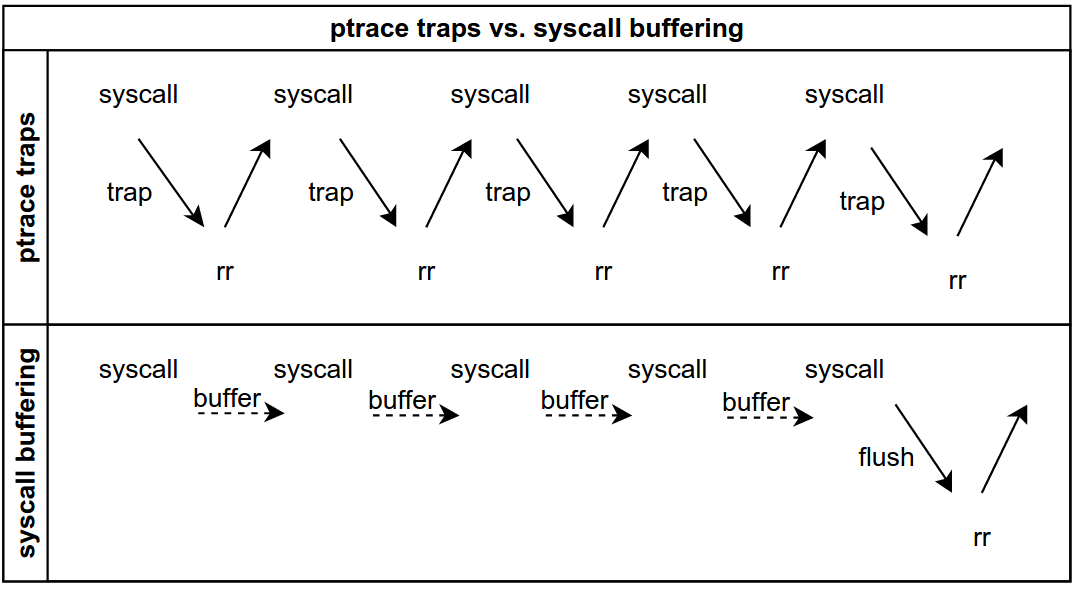
\includegraphics[scale=0.30]{Pictures/png/RR_AS}
\caption{Comparaison de l'exécution du rejeu de RR avec ptrace et seccomp-bpf
  pour gérer l'exécution des appels système.}
\label{AS_RR}
\end{figure}
Il sera utilisé pour renvoyer le bon résultat à l'application (celui sauvegardé
lors de la première phase) et gérer les autres événements de l'application
notamment les signaux et les HPC. Pour pouvoir déboguer l'application on va
utiliser les commandes gbd (placer les points d'arrêts, cotinuer
l'exécution...). En utilisant gdb à l'intérieur de son outil de débogage, RR
veut essayer de le surpasser en terme d'efficacité.

De par son fonctionnement, RR permet donc de diminuer le temps de débogage. De
plus, il peut fonctionner avec de nombreuses applications puisqu'il arrive à
gérer une grosse application telle que Firefox. Le surcoût de la phase
d'enregistrement par rapport à un simple debogage avec gdb varie selon les
applications et les tests effectués. Néanmoins, le fait que RR n'enregistre pas
la mémoire partagée en multi-tâche est un problème pour déboguer des threads. De
plus, il émule une machine simplement mono-c\oe ur ce qui est un problème pour
l'utilisation du parallélisme. Tous les appels système ne sont pas encore
implémentés et en fonction de l'application à tester on risque de voir
apparaître un problème d'interception de certains appels système exécutés par
les processus.
